\documentclass{article}

% If you're new to LaTeX, here's some short tutorials:
% https://www.overleaf.com/learn/latex/Learn_LaTeX_in_30_minutes
% https://en.wikibooks.org/wiki/LaTeX/Basics

\usepackage{subfig}

% Formatting
\usepackage[utf8]{inputenc}
\usepackage[margin=1in]{geometry}
\usepackage[titletoc,title]{appendix}
\usepackage{indentfirst}
% Math
% https://www.overleaf.com/learn/latex/Mathematical_expressions
% https://en.wikibooks.org/wiki/LaTeX/Mathematics
\usepackage{amsmath,amsfonts,amssymb,mathtools}

% Images
% https://www.overleaf.com/learn/latex/Inserting_Images
% https://en.wikibooks.org/wiki/LaTeX/Floats,_Figures_and_Captions
\usepackage{graphicx,float}

% Tables
% https://www.overleaf.com/learn/latex/Tables
% https://en.wikibooks.org/wiki/LaTeX/Tables
\usepackage{tabularx}
\usepackage{pbox}

% Algorithms
% https://www.overleaf.com/learn/latex/algorithms
% https://en.wikibooks.org/wiki/LaTeX/Algorithms
\usepackage[ruled,vlined]{algorithm2e}
\usepackage{algorithmic}


% References
% https://www.overleaf.com/learn/latex/Bibliography_management_in_LaTeX
% https://en.wikibooks.org/wiki/LaTeX/Bibliography_Management
\usepackage[citestyle=authoryear]{biblatex}
\addbibresource{bibliography.bib}

\graphicspath{{./images/}}

% Title content
\title{CSCI 350 Assignment 2}
\author{AI ID\# 520}
\date{Due: February 22, 2021}

\begin{document}

    \maketitle

    % Introduction and Overview
    \section{Depth-First Search}
        \begin{center}
            \begin{tabularx}{\textwidth}{|X|X|X|}
                \hline
                Expanded & Frontier & Associated Paths\\\hline 
                R & \{Q,S\} & \{RQ,RS\} \\\hline
                Q & \{P,U,S\} & \{RQP,RQU,RS\} \\\hline
                P & \{U,S\} & \{RQPU,RQU,RS\} \\\hline
                U & \{S\} & \{RQPUS,RQUS,RS\} \\\hline
                S & \{G1,V\} & \{RQPUSG1,RQUSG1,RQPUSV,\\&&RQUSV,RSV,RSG1\}\\\hline
                G1 & \{V\} & \{RQPUSV,RQUSV,RSV\}\\\hline
            \end{tabularx}
        \end{center}
        Order of node expansion: R-Q-P-U-S-G1\\
        Final path: R-Q-P-U-S-G1\\
    \section{Iterative Deepening Search}
        \begin{center}
            \begin{tabularx}{\textwidth}{|X|X|X|}
                \hline
                Expanded & Frontier & Associated Paths\\\hline 
                U & \{S\} & \{US\}\\\hline
                S & \{\} & end of level 1\\\hline
                U & \{S\} & \{US\}\\\hline
                S & \{G1,V\} & \{USG1,USGV\}\\\hline
                G1 & \{V\} & \{USGV\}\\\hline
            \end{tabularx}
        \end{center}
        Order of node expansion: U-S-U-S-G1\\
        Final Path: U-S-G1\\
    \section{Uniform Cost Search}
        \begin{center}
            \begin{tabularx}{\textwidth}{|X|X|X|}
                \hline
                Expanded & Frontier & Associated Paths\\\hline
                R & \{Q,S\} & \{RQ,RS\}\\\hline
                Q & \{S,P,U\} & \{RQP,RQU,RS\}\\\hline
                S & \{G1,P,U,V\} & \{RQP,RQU,RSG1,RSV\}\\\hline
                G1 & \{P,U,V,S\} & \{RQP,RQU,RSV,RSG1S\}\\\hline
            \end{tabularx}
        \end{center}
        Order of node expansion: R-Q-S-G1\\
        Final Path: R-S-G1\\[0.2in]
    \section{Breadth-First Search}
        \begin{center}
            \begin{tabularx}{\textwidth}{|X|X|X|}
                \hline
                Expanded & Frontier & Associated Paths\\\hline
                P & \{R,U\} & \{PR,PU\}\\\hline
                R & \{U,Q,S\} & \{PRQ,PRS,PU\}\\\hline
                U & \{Q,S\} & \{PRQ,PRS\}\\\hline
                Q & \{S\} & \{PRS\}\\\hline
                S & \{G1,V\} & \{PRSG1,PRSV\}\\\hline
                G1 & \{V\} & \{PRSV\}\\\hline
            \end{tabularx}
        \end{center}
        Order of node expansion: P-R-U-Q-S-G1\\
        Final Path: P-R-S-G1\\
    \section{}
        Due to the fact that node G2 has an in-degree of 0 and an out-degree of 2, its edges cannot be traversed. Consider the two possible situations, G2 is our start node and G2 is not our start node. If G2 is our start node, then we immediately find the goal and have no need to traverse either of its edges. If G2 is not our start node, then the only way to traverse the edges coming out of G2 is to somehow traverse to G2, which is not possible with its in-degree of 0.\\
    \section{}
        Please note, the changes made to the copy of agent.ipynb can be found at the bottom of the notebook, after Wumpus World.\\
            \begin{center}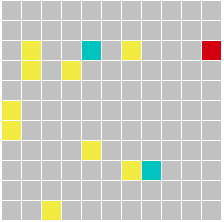
\includegraphics[width = 2in, height = 2in]{step_6.png}\end{center}

        In the above screenshot, it is clear that very little food (total of 11) and none of the water (total of 2) was consumed. During the 100 steps that were run, around half of them involved the action of turning directions at a bump. This is likely due to the fact that the agent is initially facing downward in the bottom right corner, which caused it to immediately be at a bump. From there, the only two possibilities are to turn left or right. The choices made to turn alternated, making the agent face right, then down, and so on. Being stuck in this position limited its possible moves, explaining why there were so many turns. \\

        Based on the code and my observations, the agent is very limited in its perception. It can only tell what is in its current location. When observing, this became obvious when the agent would not move towards food cells that were adjacent to it. The agent also lacks memory of its previous moves as it repeats states which do not maximize its expected utility.\\[0.7in]
    \section{}
        \begin{figure}[hbp]%
            \centering
            \subfloat[\centering First State]{{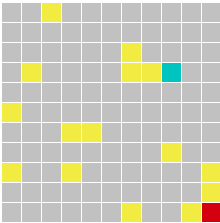
\includegraphics[width=5cm]{step_7_first.png} }}%
            \hspace{1in}%
            \subfloat[\centering Final State]{{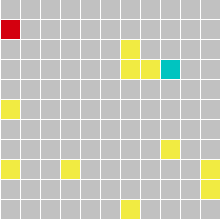
\includegraphics[width=5cm]{step_7_final.png} }}%
        \end{figure}
        This time around, I included 15 instances of food, rather than the usual 11. I also only included 1 instance of water, rather than the usual 2. During my observation of 100 steps, the agent did not get stuck in a loop of just changing directions at a bump and managed to start making its way through part of the park early on. Along the way, it was able to consume more instances of food than observed in step 6, likely due to the fact that more instances of food were available. The agent was able to move around more due to better results when choosing its action when at a bump. Early on in its steps, it made a turn in the proper direction (one which causes it to not face a bump), allowing it to have more applicable actions like move forward.
    \section{}
        \begin{figure}[hbp]%
            \centering
            \subfloat[\centering First State]{{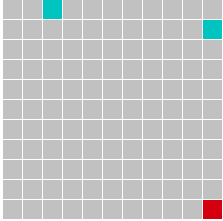
\includegraphics[width=5cm]{step_8_first.png} }}%
            \hspace{1in}%
            \subfloat[\centering Final State]{{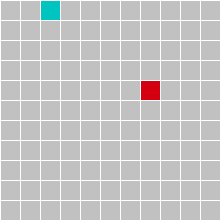
\includegraphics[width=5cm]{step_8_final.png} }}%
        \end{figure}
        Since my class code was odd, I removed all instances of food from the map. During my observation of 100 steps, I noticed that the agent's actions were to initially move closer to the water in the same column where it began. However, this is likely due to the fact that when the dog is not facing a bump, it has a higher chance of moving forward (50\%) rather than turning left (25\%) or right (25\%). In the earlier steps, it was stuck in a loop of turning left and right, causing it to constantly facing a bump. But as soon as it managed to face upwards in the last column, it began moving towards the water.\\

        From there, none of the agent's actions seemed rational. That is, its actions did not work to maximize its expected efficiency since it wandered without the appearance of a goal.\\
    \section{}
        \begin{figure}[hbp]%
            \centering
            \subfloat[\centering First State]{{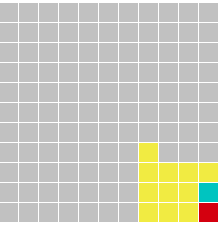
\includegraphics[width=5cm]{step_9_first.png} }}%
            \hspace{1in}%
            \subfloat[\centering Final State]{{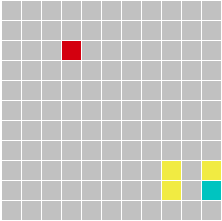
\includegraphics[width=5cm]{step_9_final.png} }}%
        \end{figure}
        Using the original settings from step 6, it would take having all of the food and water near the agent initially and having the agent consume all of the objects within its first moves. From here, since there will no longer be any food and water on the grid, the dog will eventually run out of energy and would, sadly, die.\\

        In my observation, I changed the locations of the food and water to surround the agent, with one cell of water being at the agent's initial position. During the 100 steps that were run, the agent managed to consume most of the objects that surrounded it quite fast. From there, it made a few steps towards the upper left part of the grid, and for the rest of the steps, it just wandered around there.\\

        One run is likely not enough. One run has the possibility of producing a myriad of results. Since the agent only has perception within its current location, it is not aware that it is surrounded by food and water. Therefore, it could just as easily move leftward through the bottom row, moving out of the section of food, and then roam aimlessly in the areas without food and water. Also, having multiple runs with an increasingly larger amount of steps can produce a better understanding of how this situation affects our agent. Perhaps it's unable to consume all of the objects when there is only 100 steps and therefore trying it with 500 and 1000 steps could prove beneficial. 
        
\end{document}